\documentclass[11pt, a4paper]{article}
\usepackage[labelfont=bf]{caption}
\usepackage{fancyhdr}
\usepackage{float}
\usepackage[top=25mm, right=20mm, bottom=25mm, left=20mm]{geometry}
\usepackage[hidelinks]{hyperref}
\usepackage{microtype}
\usepackage{parskip}
\usepackage{graphicx}
\usepackage{caption}

\pagestyle{fancy}
\fancyhf{}
\fancyhead[L]{COM3504}
\fancyhead[C]{The Intelligent Web: Assignment}
\fancyhead[R]{Team: Gakki}
\fancyfoot[C]{\thepage}

\begin{document}

\section{Introduction}
The Progressive Web App (PWA) allows users to create, post and search for events. WebRTC was implemented 
for users to take pictures with front and environment camera. Uploads are made available for photo 
selection from a folder. Each story can receive likes and comments which is implemented with SocketIO 
and users are able to follow one another. Attended and interested events are stored and displayed for 
each user. Web workers are used to allow offline usage with IndexedDB used to store data locally. MongoDB 
is used to store data but can only be retrieved when user is online. The search function (via location) was 
implemented with Google API, allowing selected location to be displayed on the map. For security purposes, 
users can only login with respective Google Account.

\section{Diagrams}
\begin{figure}[H]
  \begin{center}
    \begin{minipage}[b]{0.4\textwidth}
      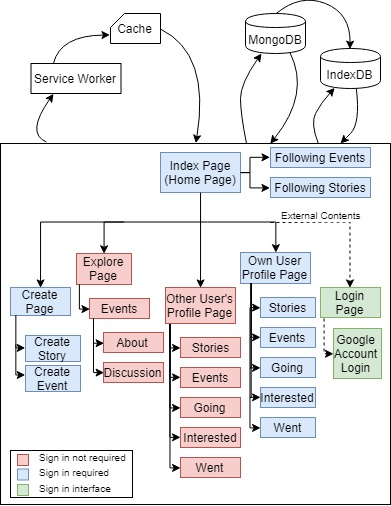
\includegraphics[width=6.8cm]{site_map.jpg}
      \caption{Demonstrates the flow of each web page in this PWA system along with the respective partial 
      pages and external content pages.}
      \label{site_map}
    \end{minipage}
    %
    \qquad
    \begin{minipage}[b]{0.4\textwidth}
      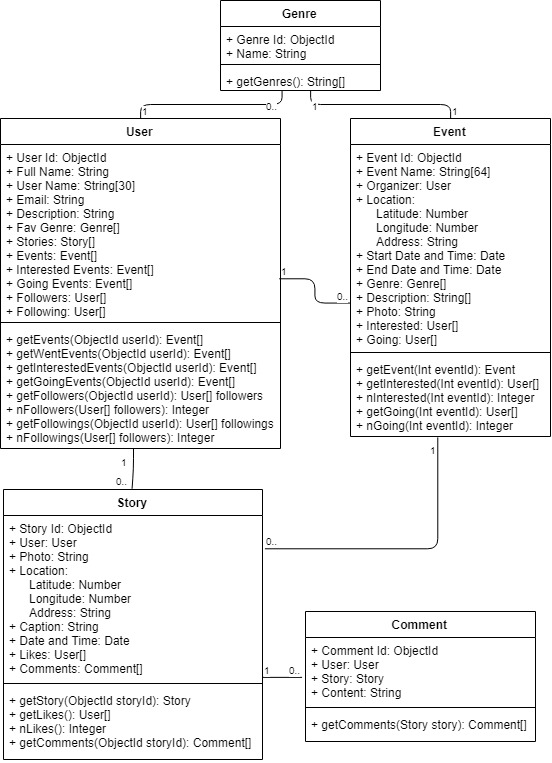
\includegraphics[width=6.8cm]{uml.jpg}
      \caption{Displays the structure of the database along with the types of content stored.}
      \label{uml}
    \end{minipage}
  \end{center}
\end{figure}
Figure~\ref{site_map} and figure~\ref{uml} are the detailed description of the PWA system structure 
with figure~\ref{site_map} describing the front-end, data storage and data retrieval, while figure~\ref{uml} 
describe the types of data stored in the database along with the relationship between the documents.

\section{Interface to Insert and Search Data via Forms}
\begin{itemize}
  \item \textbf{Challenges}: Lorem ipsum dolor sit amet, consectetur adipiscing elit. Vivamus
  bibendum turpis in sollicitudin molestie.
  \item \textbf{Solution}: Lorem ipsum dolor sit amet, consectetur adipiscing elit. Vivamus bibendum
  turpis in sollicitudin molestie.
  \item \textbf{Requirements}: Lorem ipsum dolor sit amet, consectetur adipiscing elit. Vivamus
  bibendum turpis in sollicitudin molestie.
  \item \textbf{Limitations}: Lorem ipsum dolor sit amet, consectetur adipiscing elit. Vivamus
  bibendum turpis in sollicitudin molestie.
\end{itemize}

\section{Interface to Search Data via Map}
\begin{itemize}
  \item \textbf{Challenges}: Lorem ipsum dolor sit amet, consectetur adipiscing elit. Vivamus
  bibendum turpis in sollicitudin molestie.
  \item \textbf{Solution}: Lorem ipsum dolor sit amet, consectetur adipiscing elit. Vivamus bibendum
  turpis in sollicitudin molestie.
  \item \textbf{Requirements}: Lorem ipsum dolor sit amet, consectetur adipiscing elit. Vivamus
  bibendum turpis in sollicitudin molestie.
  \item \textbf{Limitations}: Lorem ipsum dolor sit amet, consectetur adipiscing elit. Vivamus
  bibendum turpis in sollicitudin molestie.
\end{itemize}

\section{PWA – Caching of the App Template Using a Web Worker}
\begin{itemize}
  \item \textbf{Challenges}: Lorem ipsum dolor sit amet, consectetur adipiscing elit. Vivamus
  bibendum turpis in sollicitudin molestie.
  \item \textbf{Solution}: Lorem ipsum dolor sit amet, consectetur adipiscing elit. Vivamus bibendum
  turpis in sollicitudin molestie.
  \item \textbf{Requirements}: Lorem ipsum dolor sit amet, consectetur adipiscing elit. Vivamus
  bibendum turpis in sollicitudin molestie.
  \item \textbf{Limitations}: Lorem ipsum dolor sit amet, consectetur adipiscing elit. Vivamus
  bibendum turpis in sollicitudin molestie.
\end{itemize}

\section{PWA: Caching Data Using IndexedDB}
\begin{itemize}
  \item \textbf{Challenges}: Lorem ipsum dolor sit amet, consectetur adipiscing elit. Vivamus
  bibendum turpis in sollicitudin molestie.
  \item \textbf{Solution}: Lorem ipsum dolor sit amet, consectetur adipiscing elit. Vivamus bibendum
  turpis in sollicitudin molestie.
  \item \textbf{Requirements}: Lorem ipsum dolor sit amet, consectetur adipiscing elit. Vivamus
  bibendum turpis in sollicitudin molestie.
  \item \textbf{Limitations}: Lorem ipsum dolor sit amet, consectetur adipiscing elit. Vivamus
  bibendum turpis in sollicitudin molestie.

  Chrome IDB bug: disk space increases for every put
  https://github.com/google/leveldb/issues/593
  https://github.com/google/leveldb/issues/603
\end{itemize}

\section{NodeJS Server Including Non-Blocking Organisation of Multiple Dedicated Servers}
\begin{itemize}
  \item \textbf{Challenges}: Lorem ipsum dolor sit amet, consectetur adipiscing elit. Vivamus
  bibendum turpis in sollicitudin molestie.
  \item \textbf{Solution}: Lorem ipsum dolor sit amet, consectetur adipiscing elit. Vivamus bibendum
  turpis in sollicitudin molestie.
  \item \textbf{Requirements}: Lorem ipsum dolor sit amet, consectetur adipiscing elit. Vivamus
  bibendum turpis in sollicitudin molestie.
  \item \textbf{Limitations}: Lorem ipsum dolor sit amet, consectetur adipiscing elit. Vivamus
  bibendum turpis in sollicitudin molestie.
\end{itemize}

\section{MongoDB}
\begin{itemize}
  \item \textbf{Challenges}:
  \begin{itemize}
    \item Loading of initial data to populate the database.
    \item The retrieval and storage of images in the form of bits.
  \end{itemize}
  \item \textbf{Solution}:
  \begin{itemize}
    \item Initial population of database was resolved with the use of promises.
    \item Image retrieval and storage was implemented using $base64$ encoding.
  \end{itemize}
  \item \textbf{Requirements}:
  \begin{itemize}
    \item Data stored in MongoDB is stored online. Data is not stored locally and cannot be
    retrieved offline. When user is online, data is retrieved from the database and displayed on the
    PWA.
  \end{itemize}
  \item \textbf{Limitations}: Lorem ipsum dolor sit amet, consectetur adipiscing elit. Vivamus
  bibendum turpis in sollicitudin molestie.
\end{itemize}

\section{Quality of the Web Solution}
\begin{itemize}
  \item \textbf{Challenges}: Lorem ipsum dolor sit amet, consectetur adipiscing elit. Vivamus
  bibendum turpis in sollicitudin molestie.
  \item \textbf{Solution}: Lorem ipsum dolor sit amet, consectetur adipiscing elit. Vivamus bibendum
  turpis in sollicitudin molestie.
  \item \textbf{Requirements}: Lorem ipsum dolor sit amet, consectetur adipiscing elit. Vivamus
  bibendum turpis in sollicitudin molestie.
  \item \textbf{Limitations}: Lorem ipsum dolor sit amet, consectetur adipiscing elit. Vivamus
  bibendum turpis in sollicitudin molestie.
\end{itemize}

\section{Conclusions}
Lorem ipsum dolor sit amet, consectetur adipiscing elit. Vivamus bibendum turpis in sollicitudin
molestie.

\section{Division of Work}
Lorem ipsum dolor sit amet, consectetur adipiscing elit. Vivamus bibendum turpis in sollicitudin
molestie.

\section{Extra Information}
\begin{itemize}
  \item \textbf{Initial population of MongoDB}: run 'npm run initdb' to drop database and
  repopulate database with default data.
\end{itemize}

\end{document}
